\chapter{Luyện tập: Phản xạ toàn phần}
\begin{enumerate}
	\item{\textbf{(Đề chính thức của BGD-ĐT - 2018)} Chiếu một tia sáng đơn sắc từ trong nước tới mặt phân cách với không khí. Biết chiết suất của nước và của không khí đối với ánh sáng đơn sắc này lần lượt là 1,333 và 1. Góc giới hạn phản xạ toàn phần ở mặt phân cách giữa nước và không khí đối với ánh sáng đơn sắc này là 
		\begin{mcq}(4)
	\item 41,40$^\circ$.			
	\item 53,12$^\circ$.			
	\item 36,88$^\circ$.			
	\item 48,61$^\circ$.
		\end{mcq}
}	
	\item{Biết chiết suất của thủy tinh là 1,5 và của nước là $\dfrac{4}{3}$. Góc giới hạn phản xạ toàn phần khi ánh sáng truyền từ thủy tinh sang nước:
		\begin{mcq}(4)
	\item 46,8$^\circ$.			
	\item 72,5$^\circ$.			
	\item 62,7$^\circ$.			
	\item 41,8$^\circ$.
	 	\end{mcq}
}	
	\item{Một chùm tia sáng hẹp SI truyền trong mặt phẳng tiêt diện vuông góc của một khối trong suốt, đặt trong không khí, tam giác ABC vuông tại A với $\text{AB} = \text{1,2}\ \text{AC}$ như hình vẽ. Tia sáng phản xạ toàn phần ở mặt AC. Trong điều kiện đó, chiết suất n của khối trong suốt có giá trị như thế nào?
		\begin{center}
			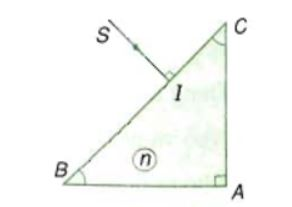
\includegraphics[scale=0.6]{../figs/VN11-PH-35-P-023-1-1.JPG}
		\end{center}
		\begin{mcq}(4)
	\item $n > \text{1,4}$.				
	\item $n < \text{1,41}$.
	\item $1 < n < \text{1,42}$.			
	\item $n > \text{1,3}$.
		\end{mcq}
}	
	\item{Một sợi quang hình trụ, lõi có chiết suất $n_1 = \text{1,50}$. Phần vỏ bọc có chiết suất $n_2 = \text{1,414}$. Chùm tia đi từ không khí tới hội tụ ở mặt trước của sợi với góc $2\alpha$ như hình vẽ. Giá trị lớn nhất của $\alpha$ để các tia sáng của chùm truyền đi được trong lõi gần giá trị nào nhất sau đây?
		\begin{center}
			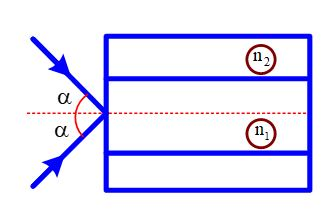
\includegraphics[scale=0.6]{../figs/VN11-PH-35-P-023-1-2.JPG}
		\end{center}
		\begin{mcq}(4)
	\item 26$^\circ$.		
	\item 60$^\circ$.			
	\item 30$^\circ$.			
	\item 41$^\circ$.
		\end{mcq}
}	
	\item{Một cái đinh được cắm vuông góc vào tâm O một tâm gỗ hình tròn có bán kính $R = 5\ \text{cm}$. Tấm gỗ được thả nổi trên mặt thoáng của một chậu nước. Đầu A của đỉnh trong nước. Cho chiết suất của nước là $n = \dfrac{4}{3}$. Để mắt không còn nhìn thấy đầu A của đỉnh thì khoảng cách OA lớn nhất là:
		\begin{mcq}(4)
	\item 6,5 cm.			
	\item 7,2 cm.			
	\item 4,4 cm.			
	\item 5,6 cm.
		\end{mcq}
}	
\end{enumerate}

\begin{center}
	\textbf{ĐÁP ÁN}
	\begin{longtable}[\textwidth]{|p{0.15\textwidth}|p{0.15\textwidth}|p{0.15\textwidth}|p{0.15\textwidth}|p{0.15\textwidth}|}
		% --- first head
		\hline%\hspace{2 pt}
		\multicolumn{1}{|c}{\textbf{Câu 1}} & \multicolumn{1}{|c|}{\textbf{Câu 2}} & \multicolumn{1}{c|}{\textbf{Câu 3}} &
		\multicolumn{1}{c|}{\textbf{Câu 4}} &
		\multicolumn{1}{c|}{\textbf{Câu 5}} \\
		\hline
		D.&C. &D. &C. &C.	\\
		\hline

		
	\end{longtable}
	
\end{center}